%%%%%%%%%%%%%%%%%%%%%%%%%%%%%%%%%%%%%%%%%%%%%%%%%%%%%%%%%%%%%%%%%%%%
%% I, the copyright holder of this work, release this work into the
%% public domain. This applies worldwide. In some countries this may
%% not be legally possible; if so: I grant anyone the right to use
%% this work for any purpose, without any conditions, unless such
%% conditions are required by law.
%%%%%%%%%%%%%%%%%%%%%%%%%%%%%%%%%%%%%%%%%%%%%%%%%%%%%%%%%%%%%%%%%%%%

\documentclass{beamer}
\usetheme[faculty=fi,logo=otinanai]{fibeamer}
\usepackage[utf8]{inputenc}
\usepackage[main=english]{babel}

%% These macros specify information about the presentation
\title{Introduction to \LaTeX} %% that will be typeset on the
\subtitle{GEO2020 - 1/12/2017} %% title page.
\author{Stelios Vitalis, Hugo Ledoux}
	
%% These additional packages are used within the document:
\usepackage{ragged2e}  % `\justifying` text
\usepackage{booktabs}  % Tables
\usepackage{tabularx}
\usepackage{tikz}      % Diagrams
\usetikzlibrary{calc, shapes, backgrounds, mindmap, trees}
\usepackage{smartdiagram}
\usepackage{amsmath, amssymb}
\usepackage{url}       % `\url`s
\usepackage{listings}  % Code listings
\lstset{language=[LaTeX]{TeX}}
\usepackage{minted}
\frenchspacing

\makeatletter
\renewcommand\fibeamer@includeLogo[1][]{}
\newcommand{\bftt}[1]{\textbf{\texttt{#1}}}
\newcommand{\comment}[1]{{\color[HTML]{008080}\textit{\textbf{\texttt{#1}}}}}
\newcommand{\cmd}[1]{{\color[HTML]{008000}\bftt{#1}}}
\newcommand{\bs}{\char`\\}
\newcommand{\cmdbs}[1]{\cmd{\bs#1}}
\newcommand{\lcb}{\char '173}
\newcommand{\rcb}{\char '175}
\newcommand{\cmdbegin}[1]{\cmdbs{begin\lcb}\bftt{#1}\cmd{\rcb}}
\newcommand{\cmdend}[1]{\cmdbs{end\lcb}\bftt{#1}\cmd{\rcb}}
\makeatother

\newcommand*\keystroke[1]{%
	\tikz[baseline=(key.base)]
	\node[%
	draw,
	fill=white,
	drop shadow={shadow xshift=0.25ex,shadow yshift=-0.25ex,fill=black,opacity=0.75},
	rectangle,
	rounded corners=2pt,
	inner sep=1pt,
	line width=0.5pt,
	font=\scriptsize\sffamily
	](key) {#1\strut}
	;
}
\newcommand{\keystrokebftt}[1]{\keystroke{\bftt{#1}}}

\newenvironment{exampletwoup}
{\VerbatimEnvironment
	\begin{VerbatimOut}{example.out}}
	{\end{VerbatimOut}
	\setlength{\parindent}{0pt}
	\fbox{\begin{tabular}{l|l}
			\begin{minipage}{0.55\linewidth}
				\inputminted[fontsize=\small,resetmargins]{latex}{example.out}
			\end{minipage} &
			\begin{minipage}{0.35\linewidth}
				\input{example.out}
			\end{minipage}
\end{tabular}}}

\newenvironment{exampletwouptiny}
{\VerbatimEnvironment
	\begin{VerbatimOut}{example.out}}
	{\end{VerbatimOut}
	\setlength{\parindent}{0pt}
	\fbox{\begin{tabular}{l|l}
			\begin{minipage}{0.55\linewidth}
				\inputminted[fontsize=\scriptsize,resetmargins]{latex}{example.out}
			\end{minipage} &
			\begin{minipage}{0.35\linewidth}
				\setlength{\parskip}{6pt plus 1pt minus 1pt}%
				\raggedright\scriptsize\input{example.out}
			\end{minipage}
\end{tabular}}}

\newenvironment{exampletwouptinynoframe}
{\VerbatimEnvironment
	\begin{VerbatimOut}{example.out}}
	{\end{VerbatimOut}
	\setlength{\parindent}{0pt}
	\begin{tabular}{l|l}
		\begin{minipage}{0.55\linewidth}
			\inputminted[fontsize=\scriptsize,resetmargins]{latex}{example.out}
		\end{minipage} &
		\begin{minipage}{0.35\linewidth}
			\setlength{\parskip}{6pt plus 1pt minus 1pt}%
			\raggedright\scriptsize\input{example.out}
		\end{minipage}
\end{tabular}}

\begin{document}
  \frame{\maketitle}

  \AtBeginSection[]{% Print an outline at the beginning of sections
    \begin{frame}<beamer>
      \frametitle{Outline for Section \thesection}
      \tableofcontents[currentsection]
    \end{frame}}

    \section{Writing Documents}
    \subsection{Good and Bad Practices}
    \begin{frame}{Typical Word Processor}
      \framesubtitle{Formatting Words}%
      \centering That's bad...
      \begin{figure}
		\includegraphics[width=0.9\textwidth]{resources/bad-practice}
      \end{figure}%
    \end{frame}
    
    \begin{frame}{Typical Word Processor}
      \framesubtitle{Using Styles}%
      \centering That's better...
      \begin{figure}
      	\includegraphics[width=0.9\textwidth]{resources/good-practice}
      \end{figure}%
    \end{frame}
    
    \subsection{Separating Content from Formatting}
    \begin{frame}{Separating Content from Formatting}
    	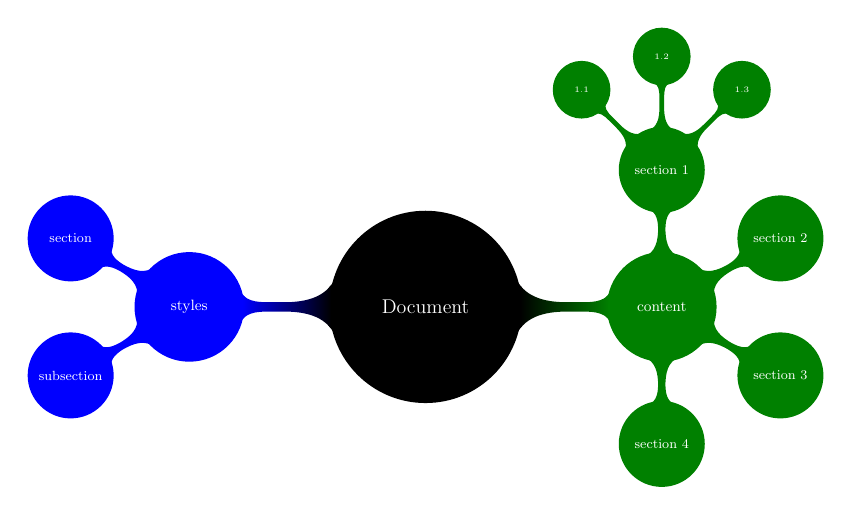
\begin{tikzpicture}[scale=0.6, every node/.style={transform shape}]
        \path[mindmap,concept color=black,text=white, level 1 concept/.append style={
      sibling angle=180}, level 2 concept/.append style={sibling angle=60}, level 3 concept/.append style={sibling angle=45}]
          node[concept] {Document}
          [clockwise from=0]
          child[concept color=green!50!black] {
            node[concept] {content}
            [clockwise from=90]
            child { node[concept] {section 1}
            	[clockwise from=135]
            	child { node[concept] {1.1} }
                child { node[concept] {1.2} }
                child { node[concept] {1.3} }
            }
            child { node[concept] {section 2} }
            child { node[concept] {section 3} }
            child { node[concept] {section 4} }
          }  
          child[concept color=blue] {
            node[concept] {styles}
            [clockwise from=210]
            child { node[concept] {subsection} }
            child { node[concept] {section} }
          };
      \end{tikzpicture}
    \end{frame}
    
    \begin{frame}{Attitude adjustment}{A new approach}
    	\begin{itemize}
        	\item Use commands to describe ``what it is'', not ``how it looks''
            \item Focus on your content
            \item Let \LaTeX\ do its job
        \end{itemize}
    \end{frame}
    
    \subsection{What is \LaTeX}
    \begin{frame}{What is \LaTeX}{The Engine}
    	\centering
        \smartdiagramset{back arrow disabled=true}
    	\smartdiagram[flow diagram:horizontal]{\LaTeX\  Code, \LaTeX\ Engine, PDF}
    \end{frame}
    
    \defverbatim[colored]\helloWorld{
      \begin{lstlisting}[tabsize=2]
  \documentclass{article}
  
  \begin{document}  
  	Hello World! % This is just comments...
  \end{document}
    \end{lstlisting}}
    \begin{frame}{Examples}{A simple document}
      \helloWorld
    \end{frame}
    
  \AtBeginSection[]{% Print an outline at the beginning of sections
	\begin{frame}<beamer>
	\frametitle{Outline for Section \thesection}
	\tableofcontents[currentsection]
\end{frame}}
    \section{Using \LaTeX}
    \subsection{Getting Started}
    \begin{frame}{Using \LaTeX}{Different options}
    	\begin{itemize}
        	\item Install it locally:
            	\begin{itemize}
                	\item A distribution (engine and packages):
                    \begin{itemize}
                        \item MiKTeX (Windows)
                        \item MacTeX (OSX)
                        \item TeXLive (Linux)
                    \end{itemize}
                    \item An Editor:
					\begin{itemize}
                        \item TexStudio (Windows, OSX, Linux)
                        \item TexMaker (Windows, OSX, Linux)
                        \item Other (\href{https://en.wikipedia.org/wiki/Comparison_of_TeX_editors}{Wikipedia Comparison})
                    \end{itemize}
                \end{itemize}
        	\item Use it online:
            	\begin{itemize}
                	\item \href{http://www.overleaf.com}{Overleaf}
                    \item \href{http://www.sharelatex.com}{ShareLatex}
                \end{itemize}
        \end{itemize}
    \end{frame}
    
        \defverbatim[colored]\simpleStructure{
      \begin{lstlisting}[tabsize=2]
  \documentclass{article}
  
  \title{A Title}
  \author{John Doe}
  
  \begin{document}
  	\maketitle
  	
  	\section{This is a section}
    Some text here.
    
    \subsection{This is a subsection}
    Some other text here.
    
    \subsection{This is another subsection}
    Guess what!
    
    This is another piece of information...
  \end{document}
  \end{lstlisting}}
    \subsection{Structure Elements}
    \begin{frame}{Examples}
    	\simpleStructure
    \end{frame}{

    \begin{frame}{Examples}{Simple Structure}
    	\includegraphics[width=0.8\textwidth]{simple-document.pdf}
    \end{frame}

\defverbatim[colored]\moreExamples{
\begin{exampletwoup}
\begin{itemize}
	\item Tea
	\item Milk
	\item Biscuits
\end{itemize}
\end{exampletwoup}
\vskip 2ex
\begin{exampletwoup}
\begin{figure}
	\includegraphics{chick}
\end{figure}
\end{exampletwoup}
\vskip 2ex
\begin{exampletwoup}
\begin{equation}
	\alpha + \beta + 1
\end{equation}
\end{exampletwoup}
}
\begin{frame}{Examples}{Structure Elements}
\moreExamples
\end{frame}

\subsection{Math}
\defverbatim[colored]\evenMoreExamples{
\begin{itemize}
	\item For the most part, you can just type your text normally.
	\begin{exampletwouptiny}
Words are separated by one or more
spaces.
		
Paragraphs are separated by one
or more blank lines.
	\end{exampletwouptiny}
	\item Space in the source file is collapsed in the output.
	\begin{exampletwouptiny}
The   rain       in Spain
falls mainly on the plain.
	\end{exampletwouptiny}
	\item Add \cmdbs{usepackage} to the pre-ample to add functionality
\end{itemize}}
\begin{frame}{Examples}{Source code}
	\evenMoreExamples    
\end{frame}

\defverbatim[colored]\mathExamples{
\begin{itemize}
	\item Why are dollar signs \keystrokebftt{\$} special? We use them to mark mathematics in text.\\[1ex]
	\begin{exampletwouptiny}
% not so good:
Let a and b be distinct positive
integers, and let c = a - b + 1.

% much better:
Let $a$ and $b$ be distinct positive
integers, and let $c = a - b + 1$.
	\end{exampletwouptiny}
\item Always use dollar signs in pairs --- one to begin the mathematics, and one
to end it.
\item \LaTeX{} handles spacing automatically; it ignores your spaces.
	\begin{exampletwouptiny}
Let $y=mx+b$ be \ldots

Let $y = m x + b$ be \ldots
	\end{exampletwouptiny}
\end{itemize}
}
\begin{frame}{Examples}{Math}
	\mathExamples
\end{frame}

\defverbatim[colored]\mathNotation{
\begin{itemize}
	\item Use caret \keystrokebftt{\^} for superscripts and underscore \keystrokebftt{\_} for subscripts.
	\begin{exampletwouptiny}
$y = c_2 x^2 + c_1 x + c_0$
	\end{exampletwouptiny}
	\vskip 2ex
	
	\item Use curly braces \keystrokebftt{\{} \keystrokebftt{\}} to group
	superscripts and subscripts.
	\begin{exampletwouptiny}
$F_n = F_n-1 + F_n-2$     % oops!

$F_n = F_{n-1} + F_{n-2}$ % ok!
	\end{exampletwouptiny}
	\vskip 2ex
	
	\item There are commands for Greek letters and common notation.
	\begin{exampletwouptiny}
$\mu = A e^{Q/RT}$

$\Omega = \sum_{k=1}^{n} \omega_k$
	\end{exampletwouptiny}
\end{itemize}}
\begin{frame}{Examples}{Math Notation}
	\mathNotation
\end{frame}

\subsection{Tables}
\defverbatim[colored]\tablesExample{
\begin{itemize}
	\item The argument specifies column alignment --- \textbf{l}eft, \textbf{r}ight, \textbf{r}ight.
	\begin{exampletwouptiny}
\begin{tabular}{lrr}
	Item   & Qty & Unit \$ \\
	Widget & 1   & 199.99  \\
	Gadget & 2   & 399.99  \\
	Cable  & 3   & 19.99   \\
\end{tabular}
	\end{exampletwouptiny}
	\item It also specifies vertical lines; use \cmdbs{hline} for horizontal lines.
	\begin{exampletwouptiny}
\begin{tabular}{|l|r|r|} \hline
	Item   & Qty & Unit \$ \\\hline
	Widget & 1   & 199.99  \\
	Gadget & 2   & 399.99  \\
	Cable  & 3   & 19.99   \\\hline
\end{tabular}
	\end{exampletwouptiny}
	\item Use an ampersand \keystrokebftt{\&} to separate columns and a double backslash \keystrokebftt{\bs}\keystrokebftt{\bs} to start a new row (like in the \bftt{align*} environment that we saw in part 1).
\end{itemize}}
\begin{frame}{Examples}{Tables}
	\tablesExample
\end{frame}

\section{References and External Programs}
\subsection{References and Bibliography}

\defverbatim[colored]\refsExamples{
\begin{itemize}{\small
		\item Use \cmdbs{label} and \cmdbs{ref} for automatic numbering.
		\item The \bftt{amsmath} package provides \cmdbs{eqref} for referencing
		equations.
}\end{itemize}
\begin{minipage}{0.55\linewidth}
	\inputminted[fontsize=\scriptsize,frame=single,resetmargins]{latex}%
	{structure-crossref.tex}
\end{minipage}
\begin{minipage}{0.35\linewidth}
	\includegraphics[width=\textwidth,clip,trim=1.8in 6in 1.6in 1in]{structure-crossref.pdf}
\end{minipage}
}
\begin{frame}{Cross-referencing}
\refsExamples
\end{frame}

\defverbatim[colored]\bibtexInfo{
\begin{itemize}
	\item Put your references in a \bftt{.bib} file in `bibtex' database format:
	\inputminted[fontsize=\scriptsize,frame=single]{latex}{bib-example.bib}
\end{itemize}}
\begin{frame}{bib\TeX}
\bibtexInfo
\end{frame}

\defverbatim[colored]\bibtexExample{
\begin{itemize}
	\item Use the \bftt{natbib} package\footnote{There is a new package with more
		features named \bftt{biblatex} but most of the articles templates still use
		\bftt{natbib}.} with \cmdbs{citet} and \cmdbs{citep}.
	\item Add \cmdbs{bibliography} and \cmdbs{bibliographystyle} at the end.
\end{itemize}
\begin{minipage}{0.55\linewidth}
	\inputminted[fontsize=\scriptsize,frame=single,resetmargins]{latex}%
	{bib-example.tex}
\end{minipage}
\begin{minipage}{0.35\linewidth}
	\includegraphics[width=\textwidth,clip,trim=1.8in 5in 1.8in 1in]{bib-example.pdf}
\end{minipage}}
\begin{frame}{bib\TeX}
\bibtexExample
\end{frame}

\begin{frame}{Manage Refereces}{External Program}
\begin{itemize}
	\item Use a tool like JabRef.
	\item All scientific websites can export to bib\TeX\ format.
	\item Save references as \bftt{.bib} file and link it from your \LaTeX\ document.
\end{itemize}
\end{frame}

\subsection{Graphics}

\begin{frame}{Designing Graphics}{Suggested Tools}
\begin{itemize}
	\item Vector graphics (Graphs, Charts, Figures):
	\begin{itemize}
		\item Adobe Illustrator (Proprietary)
		\item Inkscape (Open Source)
		\item draw.io (Free and Online)
		\item TikZ package on \LaTeX\ (for brave people)
	\end{itemize}
	\item Image Editing
	\begin{itemize}
		\item Adobe Photoshop (Proprietary)
		\item GIMP (Open Source)
	\end{itemize}
\end{itemize}
\end{frame}

\subsection{Templates}

\begin{frame}{Templates for GEO2020}{Use them as starting point}
	\begin{itemize}
		\item P2 Template: \url{https://tinyurl.com/mscgeomp2}.
		\item Final Thesis: \url{https://tinyurl.com/mscgeomthesis}.
	\end{itemize}
\end{frame}

\subsection{Exercise}
\begin{frame}{Let's do an exercise}
	Try to make the source look like the final example.
	
	\begin{itemize}
		\item Source: \url{https://tinyurl.com/latex-exerc-source}
		\item Final: \url{https://tinyurl.com/latex-exerc-final}
	\end{itemize}

\\
Your main source of information:
\begin{itemize}
	\item \url{https://en.wikibooks.org/wiki/LaTeX}
\end{itemize}
\end{frame}
\end{document}
